\item[(c)]
\section*{Exercise 3 Task (c): Qualitative Spectrum Analysis of \(x(t)\)}

\subsection*{Objective}
The objective of this task is to qualitatively visualize the spectrum of the analog signal \(x(t)\) up to 20 kHz, post conversion using a DAC with zero-order hold. This analysis focuses on how the DAC's reconstruction method impacts the signal's frequency components.

\subsection*{Methodology}
The spectrum is visualized using a plot that displays delta pulses at each significant frequency component, up to 20 kHz. The height of each pulse is modulated by the amplitude effect of the zero-order hold, which is mathematically described by the sinc function:
\[
H(f) = \frac{\sin(\pi f T)}{\pi f T}
\]
where \(T\) is the sampling period, correlating to the DAC's clock frequency of 8 kHz. This function illustrates the impact of the hold time on the spectrum's amplitude across different frequencies.

\subsection*{Results}
The plotted spectrum, as shown in the figure below, reveals several key features:
\begin{itemize}
    \item \textbf{Baseband Frequency}: The baseband component at \(1 kHz\) represents the fundamental frequency of the discrete-time signal \(x[n]\).
    Its amplitude is relatively high due to the proximity to zero frequency, where the sinc function's impact is minimal.
    \item \textbf{Harmonics and Aliasing}: Higher frequency components appear at intervals determined by the DAC's sampling rate (\(8 kHz\)). These components are noticeably attenuated and distorted due to the zero-order hold, which affects higher frequencies more significantly.
    \item \textbf{Amplitude Modulation by Sinc}: The modulation of amplitude across the spectrum due to the sinc envelope is evident, with delta pulses decreasing in height as the frequency increases away from the zero and sampling frequency multiples.
\end{itemize}
Figure~\ref{fig:exercise3c_spectrum} depicts the qualitative representation of the spectrum of \(x(t)\),
illustrating the impacts of zero-order hold and sampling frequency on the frequency components up to 20 kHz.
The delta pulses demonstrate both the presence and the relative amplitude of each component.

\begin{figure}[h]
    \centering
    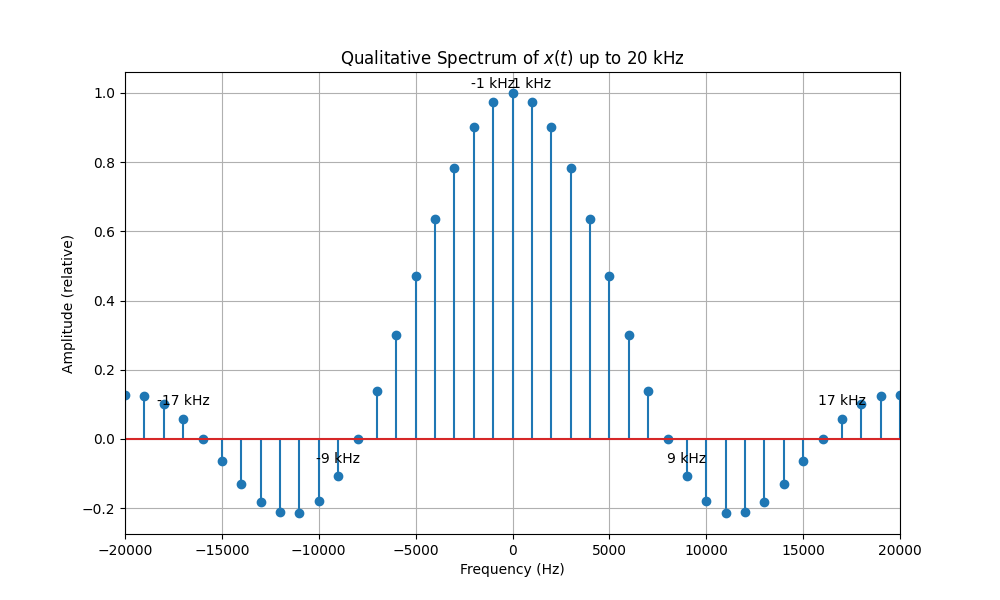
\includegraphics[width=0.8\textwidth]{fig/ex3_task_c_spectrum}
    \caption{Qualitative representation of the spectrum of \(x(t)\)}
    \label{fig:exercise3c_spectrum}
\end{figure}

\subsection*{Conclusion}
This visualization effectively demonstrates the dispersion and attenuation of frequency components due to the zero-order hold effect in DACs.
Understanding these effects is crucial for the design and analysis of digital signal processing systems, as it directly impacts the fidelity and spectral integrity of the reconstructed signal.
